\documentclass[12pt]{article}
\usepackage[margin=2.5cm]{geometry}
\usepackage{titling}
\usepackage{enumerate}
\usepackage{graphicx}
\usepackage{mdframed}
\usepackage{listings}
\usepackage{xcolor}
\usepackage[utf]{kotex}

\definecolor{codegreen}{rgb}{0,0.6,0}
\definecolor{codegray}{rgb}{0.5,0.5,0.5}
\definecolor{codepurple}{rgb}{0.58,0,0.82}
\definecolor{backcolour}{rgb}{0.95,0.95,0.92}

\lstdefinestyle{mystyle}{
    backgroundcolor=\color{backcolour},
    commentstyle=\color{codegreen},
    keywordstyle=\color{magenta},
    numberstyle=\tiny\color{codegray},
    stringstyle=\color{codepurple},
    basicstyle=\ttfamily\footnotesize,
    breakatwhitespace=false,
    breaklines=true,
    captionpos=b,
    keepspaces=true,
    numbers=left,
    numbersep=5pt,
    showspaces=false,
    showstringspaces=false,
    showtabs=false,
    tabsize=1
}

\lstset{style=mystyle}

\predate{}
\postdate{}

\begin{document}
\title{Lab 3: Inheritance}
\date{}
\maketitle

\section*{1) Play a game}

In this lab you’ll write code to play a simple number game:

\begin{itemize}
    \item This game can be played with two or more players.
    \item When the game starts, there is a count that begins at 0.
    \item On a player’s turn, they add to the count an integer that must be between a set minimum and a set maximum.
    \item The player whose move causes the count to be greater than or equal to a set goal amount is the winner.
\end{itemize}

\bigskip

\noindent Here’s a sample game with two players, where the goal is 21, the minimum move is 1, and the maximum move is 3. David is the winner.

\begin{center}
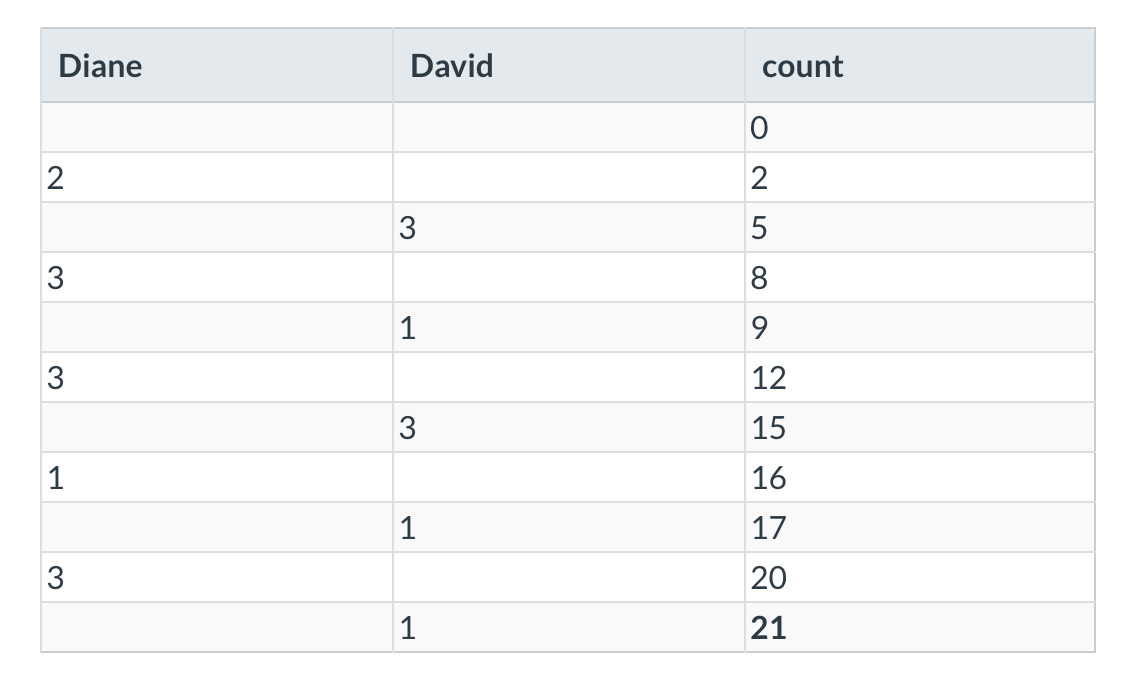
\includegraphics[width=0.8\linewidth]{../images/lab_3/table.png}
\end{center}

\bigskip

\noindent Play the game several times with your partner, using goal 21, minimum move 1,
and maximum move 3. Does a good strategy emerge?

\bigskip

\noindent (Even if it doesn’t, move on after a few minutes when you understand the game.
We’ll come back to strategies later.)

\section*{2) Become familiar with class \textit{NumberGame}}

\bigskip

Check module lab3.py the document into your lab3 folder.

\bigskip

\noindent Read the \textit{NumberGame} class carefully and answer the following questions
about it. Note that the entire class is provided for you, and your job here is
to understand it—in other words, you’re practicing your code reading skills.

\bigskip

\begin{enumerate}[1.]
    \item What attribute stores the players of the game?
    \item If \textit{turn} is 15, whose turn is it?
    \item Write a line of code that would create an instance of \textit{NumberGame}
    that violates one of the representation invariants.
    \item Which of the representation invariants is it possible to violate by
    constructing a \textit{NumberGame} improperly?
    \item List all the places in this class where a \textit{Player} is stored, an instance
    attribute of \textit{Player} is accessed or set, or a method is called on a \textit{Player}
\end{enumerate}

\bigskip

\begin{lstlisting}[language=Python,caption={lab3.py},captionpos=b]
    """CSC148 Lab 3: Inheritance

    === CSC148 Fall 2019 ===
    Department of Computer Science,
    University of Toronto

    === Module Description ===
    This module contains the implementation of a simple number game.
    The key class design feature here is *inheritance*, which is used to enable
    different types of players, both human and computer, for the game.
    """
    from __future__ import annotations
    import random
    from typing import Tuple


    class NumberGame:
        """A number game for two players.

        A count starts at 0. On a player's turn, they add to the count an amount
        between a set minimum and a set maximum. The player who brings the count
        to a set goal amount is the winner.

        The game can have multiple rounds.

        === Attributes ===
        goal:
            The amount to reach in order to win the game.
        min_step:
            The minimum legal move.
        max_step:
            The maximum legal move.
        current:
            The current value of the game count.
        players:
            The two players.
        turn:
            The turn the game is on, beginning with turn 0.
            If turn is even number, it is players[0]'s turn.
            If turn is any odd number, it is player[1]'s turn.

        === Representation invariants ==
        - self.turn >= 0
        - 0 <= self.current <= self.goal
        - 0 < self.min_step <= self.max_step <= self.goal
        """
        goal: int
        min_step: int
        max_step: int
        current: int
        players: Tuple[Player, Player]
        turn: int

        def __init__(self, goal: int, min_step: int, max_step: int,
                     players: Tuple[Player, Player]) -> None:
            """Initialize this NumberGame.

            Precondition: 0 < min_step <= max_step <= goal
            """
            self.goal = goal
            self.min_step = min_step
            self.max_step = max_step
            self.current = 0
            self.players = players
            self.turn = 0

        def play(self) -> str:
            """Play one round of this NumberGame. Return the name of the winner.

            A "round" is one full run of the game, from when the count starts
            at 0 until the goal is reached.
            """
            while self.current < self.goal:
                self.play_one_turn()
            # The player whose turn would be next (if the game weren't over) is
            # the loser. The one who went one turn before that is the winner.
            winner = self.whose_turn(self.turn - 1)
            return winner.name

        def whose_turn(self, turn: int) -> Player:
            """Return the Player whose turn it is on the given turn number.
            """
            if turn % 2 == 0:
                return self.players[0]
            else:
                return self.players[1]

        def play_one_turn(self) -> None:
            """Play a single turn in this NumberGame.

            Determine whose move it is, get their move, and update the current
            total as well as the number of the turn we are on.
            Print the move and the new total.
            """
            next_player = self.whose_turn(self.turn)
            amount = next_player.move(
                self.current,
                self.min_step,
                self.max_step,
                self.goal
            )
            self.current += amount
            self.turn += 1

            print(f'{next_player.name} moves {amount}.')
            print(f'Total is now {self.current}.')


    # TODO: Write classes Player, RandomPlayer, UserPlayer, and StrategicPlayer.


    def make_player(generic_name: str) -> Player:
        """Return a new Player based on user input.

        Allow the user to choose a player name and player type.
        <generic_name> is a placeholder used to identify which player is being made.
        """
        name = input(f'Enter a name for {generic_name}: ')
        # TODO: Create and return some sort of Player.


    def main() -> None:
        """Play multiple rounds of a NumberGame based on user input settings.
        """
        goal = int(input('Enter goal amount: '))
        minimum = int(input('Enter minimum move: '))
        maximum = int(input('Enter maximum move: '))
        p1 = make_player('p1')
        p2 = make_player('p2')
        while True:
            g = NumberGame(goal, minimum, maximum, (p1, p2))
            winner = g.play()
            print(f'And {winner} is the winner!!!')
            print(p1)
            print(p2)
            again = input('Again? (y/n) ')
            if again != 'y':
                return


    if __name__ == '__main__':
        # Uncomment the lines below to check your work using
        # python_ta and doctest.
        import python_ta
        python_ta.check_all(config={
            'extra-imports': ['random'],
            'allowed-io': [
                'main',
                'make_player',
                'move',
                'play_one_turn'
            ]
        })
        # import doctest
        # doctest.testmod()

        # Uncomment the following line to run the number game.
        # main()

\end{lstlisting}

\section*{3) Become familiar with function}

\section*{4) Plan a Player class and 3 subclasses}

\end{document}
